\documentclass[conference]{IEEEtran}
\IEEEoverridecommandlockouts

\usepackage[T1]{fontenc}
\usepackage[utf8]{inputenc}
\usepackage{cite}
\usepackage{amsmath,amssymb,amsfonts}
\usepackage{graphicx}
\usepackage{textcomp}
\usepackage{xcolor}
\usepackage{booktabs}
\usepackage{longtable}
\usepackage{array}
\usepackage{float}
\usepackage{fvextra}
\usepackage{framed}
\usepackage{hyperref}
\usepackage{calc}
\setkeys{Gin}{width=\linewidth,height=0.9\textheight,keepaspectratio}

% Pandoc may emit some Unicode punctuation/symbols directly. Map common ones for pdflatex.
\DeclareUnicodeCharacter{00B0}{\textdegree}
\DeclareUnicodeCharacter{00B2}{\textsuperscript{2}}
\DeclareUnicodeCharacter{00D7}{\ensuremath{\times}}
\DeclareUnicodeCharacter{0394}{\ensuremath{\Delta}}
\DeclareUnicodeCharacter{2013}{--}
\DeclareUnicodeCharacter{2014}{---}
\DeclareUnicodeCharacter{2019}{'}
\DeclareUnicodeCharacter{201C}{``}
\DeclareUnicodeCharacter{201D}{''}
\DeclareUnicodeCharacter{2192}{\ensuremath{\rightarrow}}
\DeclareUnicodeCharacter{21D2}{\ensuremath{\Rightarrow}}
\DeclareUnicodeCharacter{2248}{\ensuremath{\approx}}

\def\BibTeX{{\rm B\kern-.05em{\sc i\kern-.025em b}\kern-.08em
    T\kern-.1667em\lower.7ex\hbox{E}\kern-.125emX}}

\hypersetup{hidelinks}
\definecolor{shadecolor}{gray}{0.95}

% Pandoc emits \tightlist for compact lists in some outputs.
\providecommand{\tightlist}{%
  \setlength{\itemsep}{0pt}\setlength{\parskip}{0pt}}
% Pandoc 3.2+ wraps figures in \pandocbounded; no-op shim for templates that don't define it.
\providecommand{\pandocbounded}[1]{#1}

% Support for Pandoc --citeproc output.
\newlength{\cslhangindent}
\setlength{\cslhangindent}{1.5em}
\newlength{\csllabelwidth}
\setlength{\csllabelwidth}{3em}
\providecommand{\citeproctext}{}
\newenvironment{CSLReferences}[2] % #1 hanging indent (ignored), #2 entry spacing
  {\begin{list}{}{%
     \setlength{\leftmargin}{\csllabelwidth}%
     \setlength{\labelwidth}{\csllabelwidth}%
     \setlength{\labelsep}{0pt}%
     \setlength{\itemindent}{0pt}%
     \setlength{\itemsep}{#2\baselineskip}%
     \setlength{\parsep}{0pt}%
   }}
  {\end{list}}
\newcommand{\CSLBlock}[1]{#1\par}
\newcommand{\CSLLeftMargin}[1]{\parbox[t]{\csllabelwidth}{#1}}
\newcommand{\CSLRightInline}[1]{\parbox[t]{\linewidth - \csllabelwidth}{#1}}
\newcommand{\CSLIndent}[1]{\hspace{\cslhangindent}#1}

\usepackage{color}
\usepackage{fancyvrb}
\newcommand{\VerbBar}{|}
\newcommand{\VERB}{\Verb[commandchars=\\\{\}]}
\DefineVerbatimEnvironment{Highlighting}{Verbatim}{commandchars=\\\{\}}
% Add ',fontsize=\small' for more characters per line
\newenvironment{Shaded}{}{}
\newcommand{\AlertTok}[1]{\textcolor[rgb]{1.00,0.00,0.00}{\textbf{#1}}}
\newcommand{\AnnotationTok}[1]{\textcolor[rgb]{0.38,0.63,0.69}{\textbf{\textit{#1}}}}
\newcommand{\AttributeTok}[1]{\textcolor[rgb]{0.49,0.56,0.16}{#1}}
\newcommand{\BaseNTok}[1]{\textcolor[rgb]{0.25,0.63,0.44}{#1}}
\newcommand{\BuiltInTok}[1]{\textcolor[rgb]{0.00,0.50,0.00}{#1}}
\newcommand{\CharTok}[1]{\textcolor[rgb]{0.25,0.44,0.63}{#1}}
\newcommand{\CommentTok}[1]{\textcolor[rgb]{0.38,0.63,0.69}{\textit{#1}}}
\newcommand{\CommentVarTok}[1]{\textcolor[rgb]{0.38,0.63,0.69}{\textbf{\textit{#1}}}}
\newcommand{\ConstantTok}[1]{\textcolor[rgb]{0.53,0.00,0.00}{#1}}
\newcommand{\ControlFlowTok}[1]{\textcolor[rgb]{0.00,0.44,0.13}{\textbf{#1}}}
\newcommand{\DataTypeTok}[1]{\textcolor[rgb]{0.56,0.13,0.00}{#1}}
\newcommand{\DecValTok}[1]{\textcolor[rgb]{0.25,0.63,0.44}{#1}}
\newcommand{\DocumentationTok}[1]{\textcolor[rgb]{0.73,0.13,0.13}{\textit{#1}}}
\newcommand{\ErrorTok}[1]{\textcolor[rgb]{1.00,0.00,0.00}{\textbf{#1}}}
\newcommand{\ExtensionTok}[1]{#1}
\newcommand{\FloatTok}[1]{\textcolor[rgb]{0.25,0.63,0.44}{#1}}
\newcommand{\FunctionTok}[1]{\textcolor[rgb]{0.02,0.16,0.49}{#1}}
\newcommand{\ImportTok}[1]{\textcolor[rgb]{0.00,0.50,0.00}{\textbf{#1}}}
\newcommand{\InformationTok}[1]{\textcolor[rgb]{0.38,0.63,0.69}{\textbf{\textit{#1}}}}
\newcommand{\KeywordTok}[1]{\textcolor[rgb]{0.00,0.44,0.13}{\textbf{#1}}}
\newcommand{\NormalTok}[1]{#1}
\newcommand{\OperatorTok}[1]{\textcolor[rgb]{0.40,0.40,0.40}{#1}}
\newcommand{\OtherTok}[1]{\textcolor[rgb]{0.00,0.44,0.13}{#1}}
\newcommand{\PreprocessorTok}[1]{\textcolor[rgb]{0.74,0.48,0.00}{#1}}
\newcommand{\RegionMarkerTok}[1]{#1}
\newcommand{\SpecialCharTok}[1]{\textcolor[rgb]{0.25,0.44,0.63}{#1}}
\newcommand{\SpecialStringTok}[1]{\textcolor[rgb]{0.73,0.40,0.53}{#1}}
\newcommand{\StringTok}[1]{\textcolor[rgb]{0.25,0.44,0.63}{#1}}
\newcommand{\VariableTok}[1]{\textcolor[rgb]{0.10,0.09,0.49}{#1}}
\newcommand{\VerbatimStringTok}[1]{\textcolor[rgb]{0.25,0.44,0.63}{#1}}
\newcommand{\WarningTok}[1]{\textcolor[rgb]{0.38,0.63,0.69}{\textbf{\textit{#1}}}}

\RecustomVerbatimEnvironment{Highlighting}{Verbatim}{
  commandchars=\\\{\},
  breaklines,
  breakanywhere=true,
  breaksymbolleft={},
  fontsize=\footnotesize
}
\renewenvironment{Shaded}{\begin{snugshade}}{\end{snugshade}}


\begin{document}

\title{Modality-Driven Search with Holistic Trace Judging for ARC-AGI-2}

\author{
  \IEEEauthorblockN{Johan Land}
  \IEEEauthorblockA{Independent Researcher \\
  johan.land@gmail.com}
}

\maketitle

\begin{abstract}
Large language models can produce fluent, internally coherent reasoning
traces for abstract reasoning tasks while still being confidently wrong
--- making selection among candidates, not just generation, the central
challenge. I present a solver for ARC-AGI-2 (a few-shot visual reasoning
benchmark) built around two principles: (i) treating reasoning
modalities as search operators, generating diverse candidates
independently across text, image, and code channels, and (ii)
context-preserving holistic judging, in which a judge model jointly
compares all candidate reasoning traces within a single long-context
prompt. Unlike self-consistency or majority voting, this approach
reliably recovers correct minority hypotheses on tasks where the modal
answer is wrong.

On the ARC Prize semi-private evaluation set, the solver achieves 72.9\%
at \$38.99/task --- the highest score on the verified leaderboard at the
time of writing, exceeding the best standalone frontier models (GPT-5.2
Pro at 54.2\%, Gemini 3 Pro at 54.0\%) by +18.7 percentage points. On
the public evaluation set, it achieves 76.1\% at \$19.69/task. I release
the full source code and document extensive negative results, including
the finding that prescriptive prompting templates and iterative
refinement systematically reduce hypothesis diversity and degrade
performance.
\end{abstract}

\begin{IEEEkeywords}
ARC, ARC-AGI-2, large language models, multimodal reasoning, program
synthesis, LLM-as-a-judge
\end{IEEEkeywords}

\section{Introduction}\label{introduction}

A central challenge in applying LLMs to abstract reasoning is not just
producing candidate solutions, but \textbf{knowing what is right and
what is wrong} in a setting where models can be confidently
incorrect---even when they provide detailed, plausible reasoning traces.

ARC-AGI-2 was designed to be \emph{easy for humans and hard for AI},
and---critically---to measure both \textbf{capability} and
\textbf{efficiency} (cost). Progress on ARC-style benchmarks has been
rapid: ARC Prize reports significant year-over-year improvements driven
by frontier reasoning systems and application-layer refinement harnesses
{[}1{]}.

This paper describes an ARC-AGI-2 solver that treats \textbf{modalities
as search operators} and uses \textbf{judging as the final selection
mechanism}: generate diverse candidate solutions across independent
reasoning channels, then select among them using context-preserving
holistic judging.\footnote{An extended version of this paper with
  complete failure analysis, task-level breakdowns, judge rationale
  transcripts, and additional ablation details is available as a
  preprint {[}2{]}.}

\subsection{Contributions}\label{contributions}

\begin{itemize}
\tightlist
\item
  \textbf{A modality-driven search solver for ARC-AGI-2} that generates
  candidates independently across text, image, and code reasoning
  channels.
\item
  \textbf{A context-preserving holistic judge in this setting} that
  reads all candidate traces jointly to select the best outputs,
  identifying correct \emph{minority} hypotheses---yielding +7 solved
  instances over majority vote at only 13\% of total system cost
  (Section V).
\item
  \textbf{Verified ARC-AGI-2 semi-private performance:} 72.9\% at
  \$38.99/task on the ARC Prize Verified leaderboard\footnote{https://arcprize.org/leaderboard}---the
  highest score on the leaderboard at the time of writing, exceeding the
  best standalone frontier models (GPT-5.2 Pro at 54.2\%, Gemini 3 Pro
  at 54.0\%) by +18.7 percentage points.
\item
  \textbf{Public eval performance:} 76.11\% at \$19.69/task
  (self-measured).
\item
  \textbf{Open-source release} of the full source code, detailed
  negative results, and complete public-evaluation run data to support
  future research.
\end{itemize}

\begin{center}\rule{0.5\linewidth}{0.5pt}\end{center}

\section{Background and Related Work}\label{background-and-related-work}

The Abstraction and Reasoning Corpus (ARC) was introduced by {[}3{]} as
a benchmark for measuring intelligence as skill-acquisition
efficiency---how effectively a system acquires new skills under
constrained experience and priors. Tasks are framed as few-shot
input--output induction over grids: given a handful of training
demonstration pairs, the solver must infer an underlying transformation
rule and apply it to a held-out test input. ARC-AGI-2 {[}1{]} extends
the original benchmark with harder tasks, formalized dataset splits
(training, public, semi-private, and private evaluation sets of
calibrated tasks), pass@2 scoring, first-party human calibration, and an
emphasis on both accuracy and cost efficiency. Fig. 2 illustrates a
representative task.

\begin{figure}
\centering
\pandocbounded{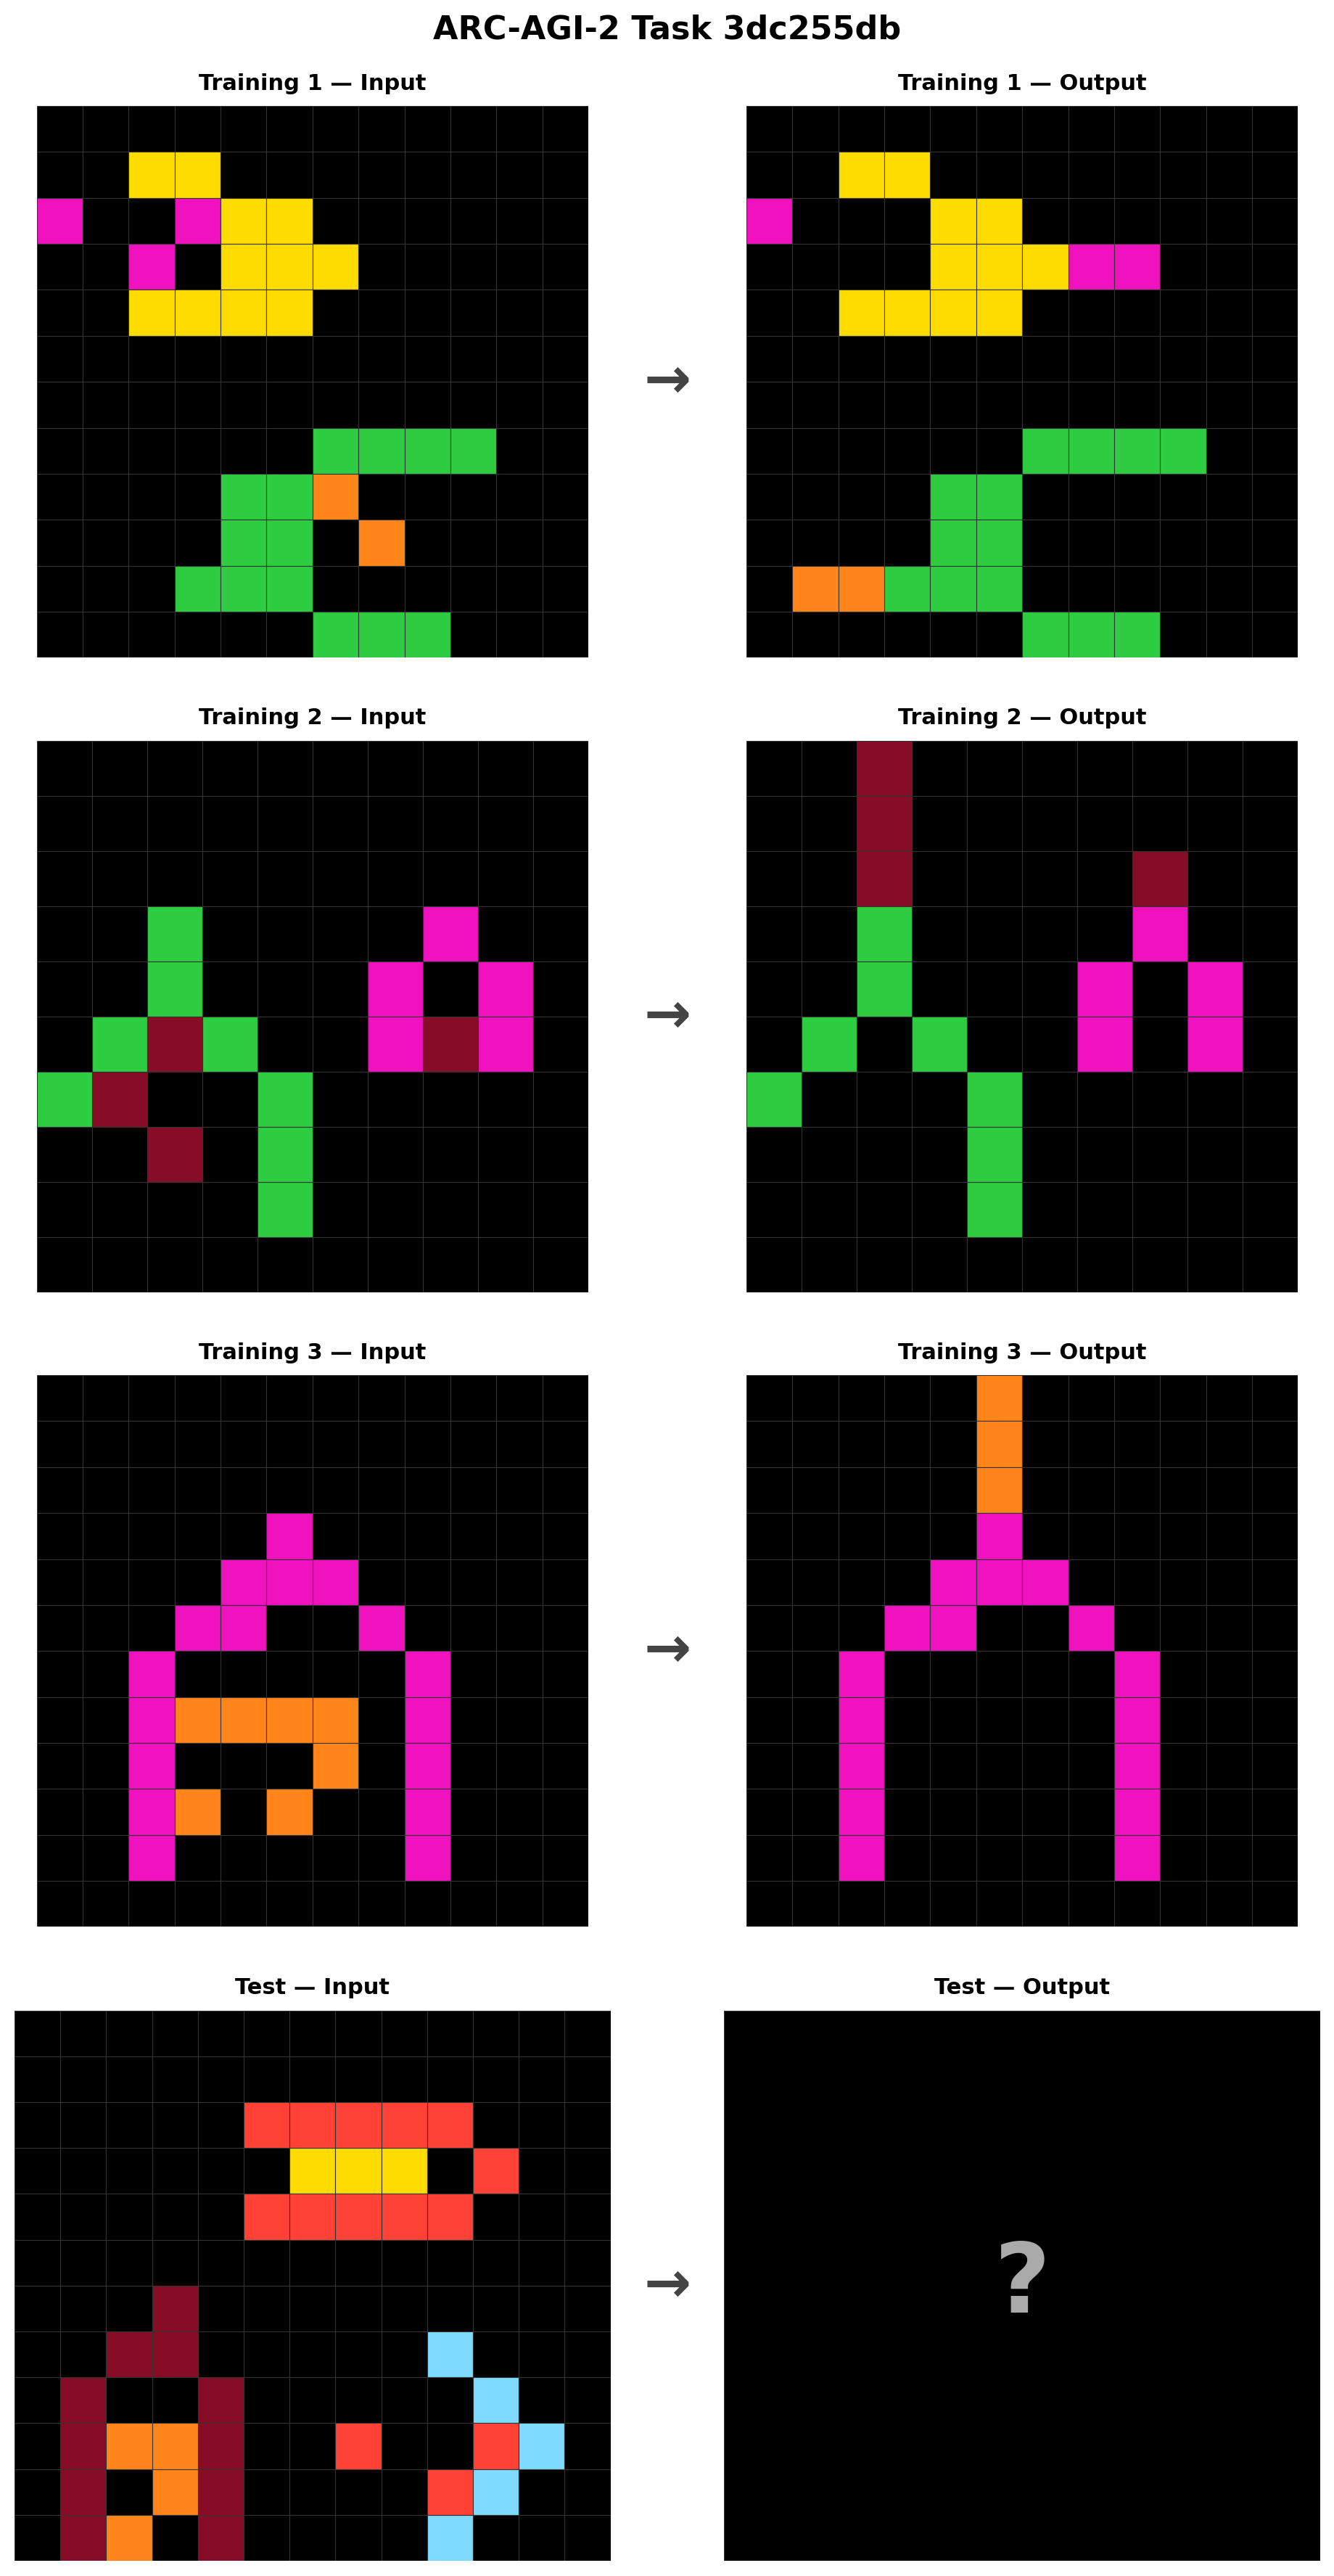
\includegraphics[keepaspectratio,alt={ARC-AGI-2 task 3dc255db. A human might see ``spaceships'' with particles on the exhaust side. The transformation removes the particles from the interior and extends them from the nose. Three training pairs (rows 1--3) demonstrate the rule; the test input (row 4) must be solved from these examples alone. This task remains unsolved by the system.}]{figures/task_example.png}}
\caption{ARC-AGI-2 task \protect\texttt{3dc255db}. A human might see
``spaceships'' with particles on the exhaust side. The transformation
removes the particles from the interior and extends them from the nose.
Three training pairs (rows 1--3) demonstrate the rule; the test input
(row 4) must be solved from these examples alone. This task remains
unsolved by the system.}
\end{figure}

Classical ARC solvers treat tasks as latent programs composed from a
hand-designed DSL {[}4{]}. Learned approaches attack ARC via induction
or transduction; {[}5{]} show that ensembling both paradigms can
approach human-level performance. Test-time adaptation has emerged as a
major axis: {[}6{]} demonstrate that updating model parameters at test
time yields strong gains, while {[}7{]} combine learned representations
with explicit program search.

The broader LLM literature has developed test-time compute techniques
directly relevant to this work. Chain-of-thought prompting {[}8{]}
elicits intermediate reasoning steps; self-consistency {[}9{]} samples
multiple paths and selects the most common answer. Tree of Thoughts
{[}10{]} reframes inference as search with branching and backtracking.
ReAct {[}11{]} interleaves reasoning with tool calls, and PAL {[}12{]}
translates problems into executable code. Iterative-refinement methods
{[}13{]}, {[}14{]} improve outputs through feedback loops but risk
anchoring to early hypotheses. {[}15{]} show that optimally allocating
test-time compute can be more effective than scaling model parameters.

Relative to this landscape, the present work composes three trends: (i)
hypothesis generation as explicit search across \emph{multiple reasoning
modalities}, extending ToT-style inference {[}10{]}; (ii) tool- and
program-mediated reasoning {[}11{]}, {[}12{]} used to produce richer
intermediate artifacts for downstream selection; and (iii) judge-based
selection adapted from the LLM-as-a-judge paradigm {[}16{]}. What is
distinctive is the combination of heterogeneous candidate generators
with context-preserving comparison over full reasoning traces, rather
than scalar scoring or consensus compression.

\begin{center}\rule{0.5\linewidth}{0.5pt}\end{center}

\section{Method}\label{method}

The solver is built around a practical observation: to solve tasks that
frontier systems do not already solve, the correct solution is often a
\textbf{minority hypothesis}. If the most common solution were correct,
the task would likely already be within the main cluster of model
behavior. The solver's first phase therefore creates many
\emph{independent} candidate solutions across heterogeneous reasoning
modalities (text, image, and code), maximizing the probability that at
least one candidate captures a genuinely novel hypothesis. Each modality
provides a structurally different representation of the same task, which
empirically produces candidates that cluster differently (Section IV-E).

\subsection{Pipeline Overview}\label{pipeline-overview}

Fig. 2 shows the end-to-end pipeline. For each ARC task:

\begin{figure}
\centering
\pandocbounded{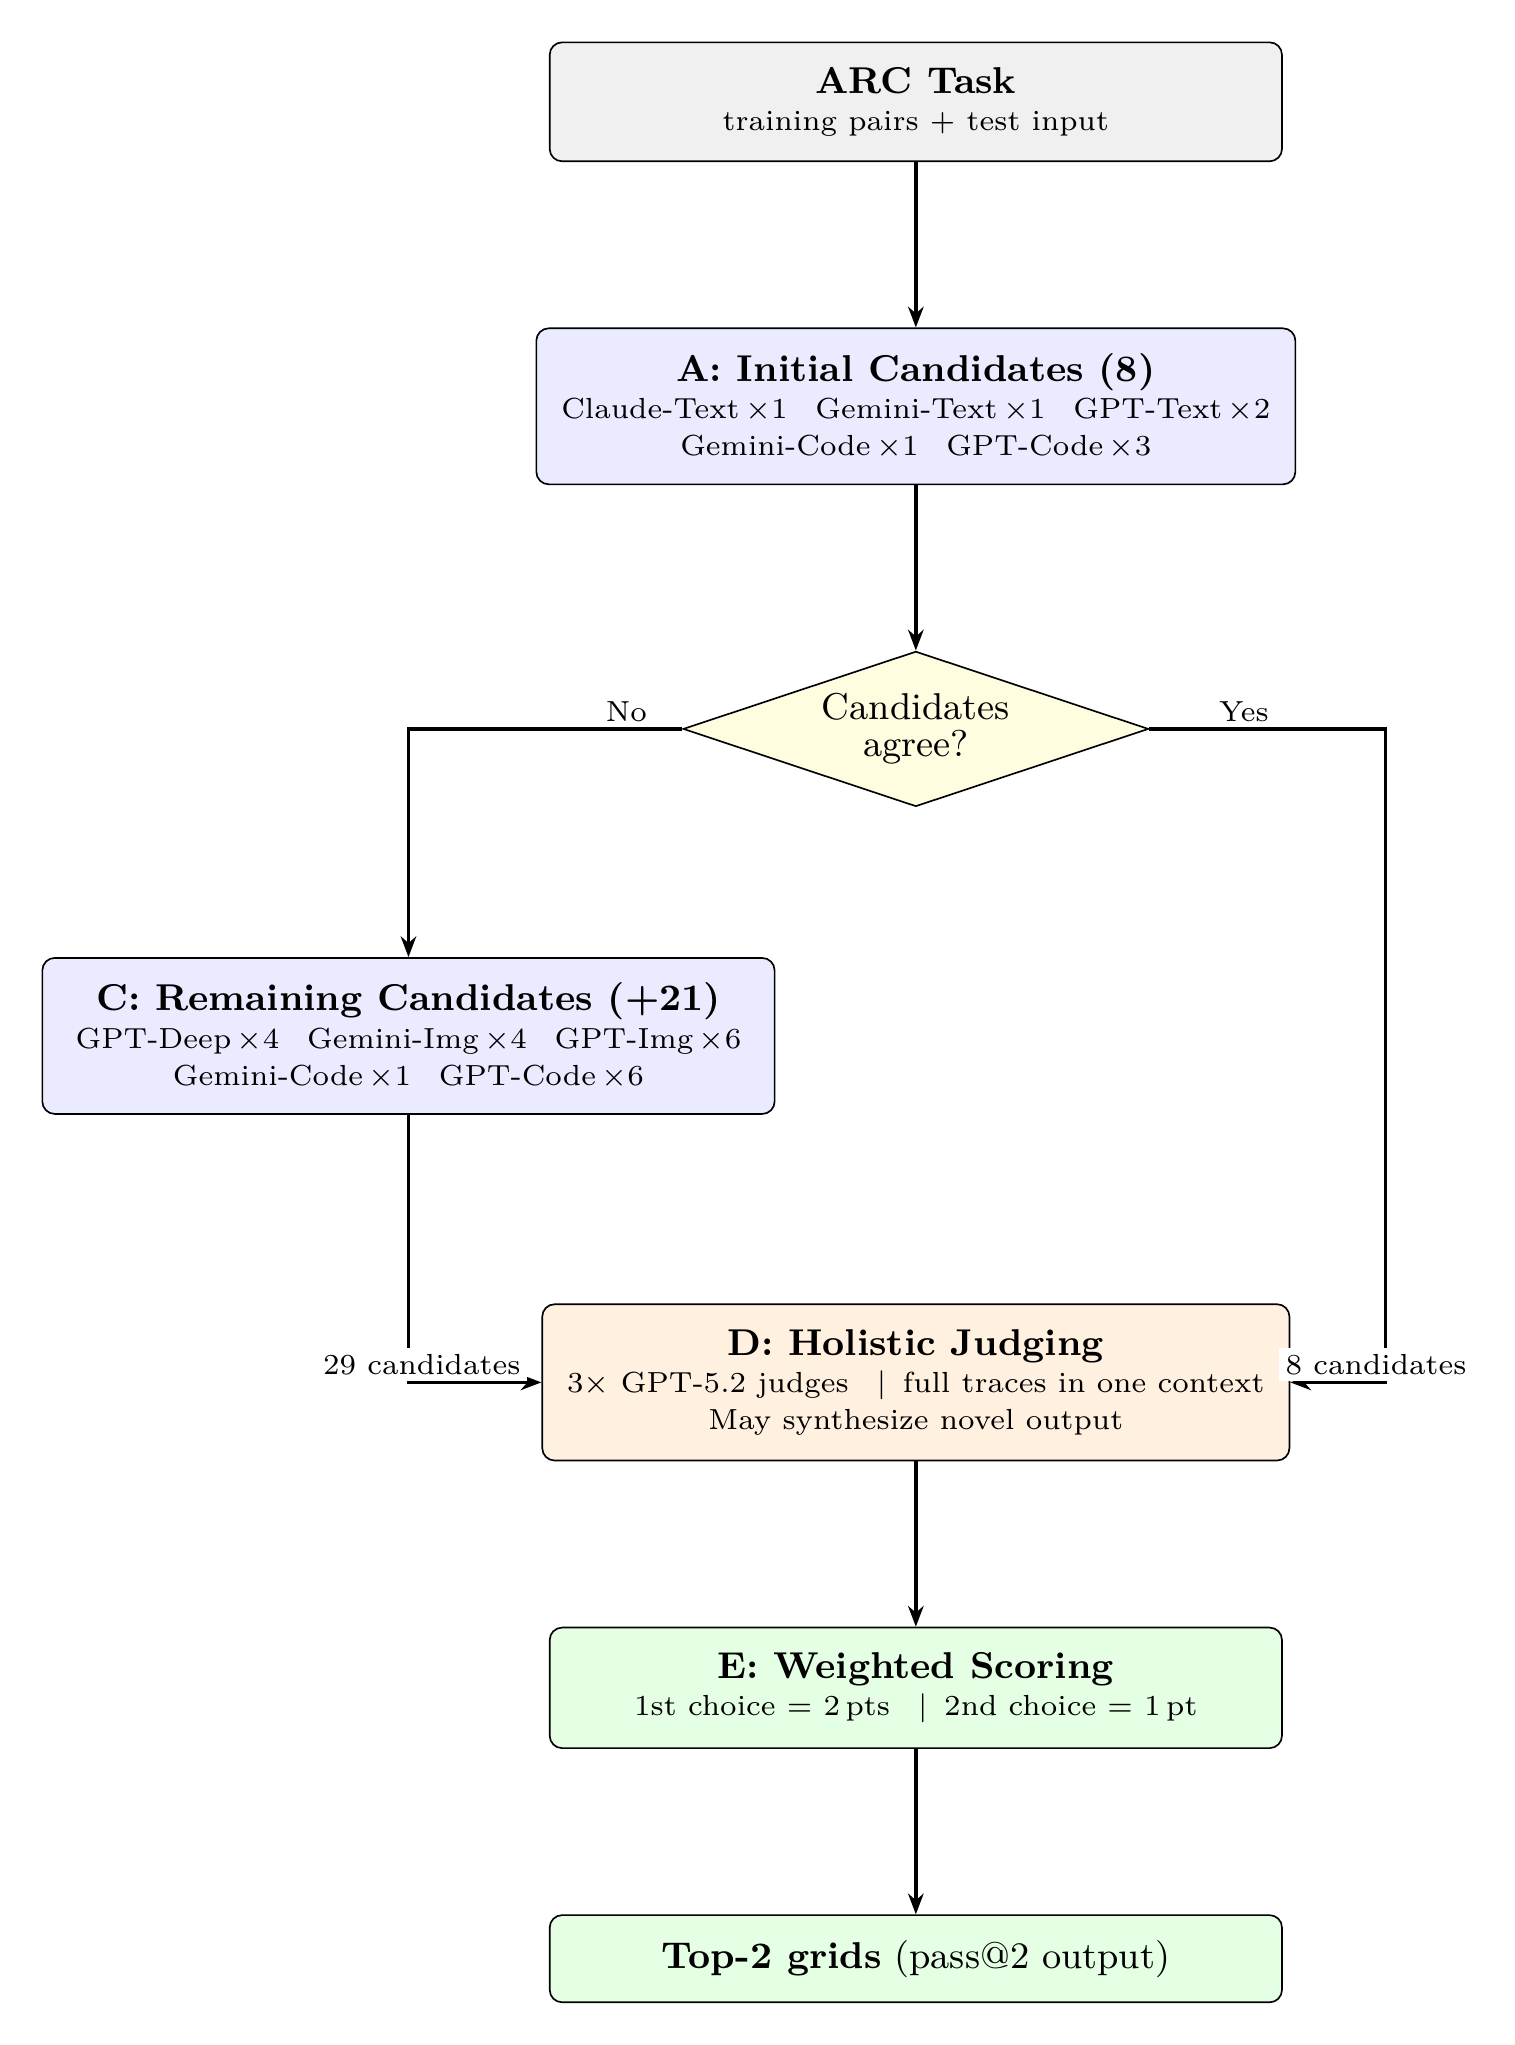
\includegraphics[keepaspectratio,alt={System pipeline overview.}]{figures/pipeline.png}}
\caption{System pipeline overview.}
\end{figure}

\begin{enumerate}
\def\labelenumi{\arabic{enumi}.}
\item
  \textbf{Candidate generation (up to 29 candidates).} A set of
  modality-specific solvers is run, each producing a predicted output
  grid, a reasoning trace, and, for code candidates, the code plus
  tool-use logs. Each candidate produces one output; the pass@2
  two-guess format is introduced only at the judging stage. Candidate
  generation proceeds in stages: if early candidates already show strong
  agreement, the system terminates early and skips the remaining, more
  expensive modalities. This adaptive early stopping improves cost
  efficiency on tasks that can be solved with a shallower search. On the
  ARC-AGI-2 public evaluation, 37 of 167 instances stopped after the
  initial 8-candidate probe, and \textbf{36 of those 37 were solved
  correctly} (97.3\%), showing that shallow search is often sufficient
  on easier tasks. The same principle is even more effective on easier
  ARC-AGI-1 tasks, where the system achieves 94.5\% on the official
  semi-private evaluation at only \$11.40/task, substantially cheaper
  than the \$38.99/task on ARC-AGI-2. Both semi-private scores and costs
  are as reported by ARC Prize's verification infrastructure. The single
  early-stopping failure (\texttt{dbff022c:1}) is a case of extreme
  groupthink: all models confidently assume the simpler of two valid
  legend-to-color interpretations while the ground truth requires the
  more complex one. This validates the heuristic on easy tasks, but also
  shows that early consensus can mask genuine ambiguity.
\item
  \textbf{Holistic judging (3 parallel judges).} All candidate traces
  are concatenated into a single long-context prompt. Each judge model
  is asked to identify the top-2 most likely correct candidates (or
  propose a synthesis that recombines correct subcomponents), explain
  why other candidate clusters are wrong, and output the final grids.
\item
  \textbf{Weighted scoring.} Each judge's first choice receives 2 points
  and second choice receives 1 point. The system sums points across
  judges for each distinct output grid. The two grids with the highest
  total score become the solver's pass@2 guesses.
\end{enumerate}

ARC-AGI-2 tasks often introduce new concepts that were not exercised in
the training pairs. A solution can be perfectly ``logical'' on the
training examples but still be a brittle overfit that fails to abstract
the intended rule. This makes naive logic checking of traces
insufficient (Sections III-C and VI). In practice, the system needs
broad hypothesis exploration across structurally different
representations, combined with a judge that can identify \textbf{where}
a candidate is likely overfitting --- even when its reasoning reads as
coherent.

\begin{center}\rule{0.5\linewidth}{0.5pt}\end{center}

\subsection{Multimodal Candidate
Generation}\label{multimodal-candidate-generation}

Candidate generation is performed via three foundation models across
multiple inference configurations: \textbf{Gemini 3 Preview} in a
high-reasoning setting (text, image, and code with tools),
\textbf{GPT-5.2} in an x-high reasoning setting (text, image, code with
and without tools, and a deep-think configuration), and \textbf{Claude
Opus 4.5} in a long-context (120k) setting (text reasoning). Exact API
parameters, tool schemas, and prompts are documented in the open-source
implementation. In the final system, generators are grouped into three
families --- \textbf{Text}, \textbf{Image}, and \textbf{Code} --- with
multiple configurations within each family to encourage diversity. Table
I shows the full candidate configuration.

\begin{table}[htbp]
\caption{Candidate configuration: 29 generators grouped by family.}
\begin{center}
\footnotesize
\begin{tabular}{|l|l|c|}
\hline
\textbf{Family} & \textbf{Generator} & \textbf{Candidates} \\
\hline
Text & Claude Opus 4.5 (text) & 1 \\
Text & Gemini 3 Preview (text) & 1 \\
Text & GPT-5.2 (text) & 2 \\
Text & GPT-5.2 (deep think) & 4 \\
Image & Gemini 3 Preview (image) & 4 \\
Image & GPT-5.2 (image) & 6 \\
Code & Gemini 3 Preview (code, tools) & 2 \\
Code & GPT-5.2 (code, tools) & 9 \\
\hline
\multicolumn{2}{|r|}{\textbf{Total}} & \textbf{29} \\
\hline
\end{tabular}
\end{center}
\end{table}

The text family contributes 8 candidates (including 4 deep-think runs),
image contributes 10, and code contributes 11. Within each family,
multiple runs of the same generator use the same prompt and API
parameters; diversity arises from model sampling stochasticity.

\textbf{Text methodology.} Text candidates are generated by prompting a
language model with a textual encoding of the ARC training pairs and
test input. The model is asked to infer the transformation rule and
output a completed test grid. The base prompt is intentionally minimal:

\begin{Shaded}
\begin{Highlighting}[]
\NormalTok{You are solving an ARC task. Each grid cell is an integer}
\NormalTok{0{-}9 representing a color. Use the solved examples to infer}
\NormalTok{the transformation and apply it to the test input.}
\NormalTok{\{training and test examples\}}
\NormalTok{Respond with an explanation of your thinking ... you MUST}
\NormalTok{also respond with the completed output grid.}
\end{Highlighting}
\end{Shaded}

The prompt deliberately does not prescribe a fixed reasoning template,
step-by-step plan, or output format, which reduces compliance overhead
and empirically increases hypothesis diversity. The trade-off is noisier
outputs that require tolerant parsing and validation to recover
candidate grids (see Section VI for negative results on prescribed
reasoning templates). Grids are encoded in CSV format, selected after
benchmarking multiple representation formats; suboptimal format choices
cost on the order of 10\% lost performance.

\textbf{``Deep think'' variant.} In addition to the standard text
prompt, a ``deep think'' configuration allocates a larger test-time
compute budget by explicitly encouraging GPT-5.2 to reason more
extensively before committing to a final output --- effectively trading
tokens for deeper deliberation within a single response. This accounts
for 4 of the 8 text candidates (Table I).

\textbf{Image methodology.} Image candidates are generated by rendering
the ARC training pairs and test input as a single annotated image
alongside a textual instruction prompt. This provides the model with a
pixel-space representation that can be advantageous for tasks where
salient structure is more readily perceived visually than through a
textual grid encoding. The image renderings are intentionally
\textbf{imprecise} --- slightly distorted rather than pixel-perfect grid
reproductions. Pixel-perfect renderings underperformed in early
experiments, possibly because models treated them as lossless encodings
and fell back on cell-by-cell numerical reasoning rather than engaging
the visual pattern recognition that makes image prompting valuable. The
slight imprecision appears to encourage models to reason about shapes,
symmetries, and spatial relationships at a higher level of abstraction.
In the public evaluation analysis (Section IV-E), image prompting
provides uniquely correct candidates on several instances.

\textbf{Code methodology.} Code candidates treat ARC solving as program
synthesis: the model is asked to produce executable code that maps input
grids to output grids. Two code-generation regimes are used.
\emph{Tool-integrated code generation} lets the model iteratively write
code, execute it via a sandbox tool, inspect intermediate outputs, and
refine the program across multiple tool calls;\footnote{The ARC Prize
  semi-private evaluation uses OpenAI's zero-data-retention (ZDR) API
  mode, which disables tool calls. For the semi-private run,
  tool-integrated code candidates were replaced with one-shot code
  generation.} this regime often produces rich intermediate artifacts
(program drafts, test harnesses, execution traces) that are later
consumed by the holistic judge. \emph{One-shot code generation} returns
a complete program in a single response without iterative feedback ---
substantially cheaper but less robust on tasks that benefit from
iterative debugging. The tool-integrated regime is the primary code
strategy, contributing the majority of code candidates.

\begin{center}\rule{0.5\linewidth}{0.5pt}\end{center}

\subsection{Context-Preserving Holistic
Judging}\label{context-preserving-holistic-judging}

Given 8--29 candidates per task, many are plausible and internally
coherent. Worse, models tend to \textbf{cluster} around the same wrong
interpretation on the hardest tasks. The key difficulty is identifying a
rare candidate that is correct --- or close enough that it can be
repaired --- without reducing everything to an overly lossy score. Three
judging approaches were tested:

\begin{enumerate}
\def\labelenumi{\arabic{enumi}.}
\tightlist
\item
  \textbf{Logic judge (failed):} Scoring candidates by whether their
  reasoning appears logically consistent fails because a candidate can
  be internally coherent yet overfit to training pairs or miss a latent
  concept introduced in the test case.
\item
  \textbf{Consistency judge (partial):} Selecting themes that repeat
  across candidates rewards the majority cluster, but breaking new
  ground requires elevating \emph{divergent} hypotheses --- the correct
  solution to an unsolved task is often not the modal answer.
\item
  \textbf{Holistic judge (final):} All traces are provided
  \emph{together} in a single prompt, and the judge picks the top-2 most
  likely correct candidates. Three judges run in parallel and their
  picks are aggregated via weighted scoring. This works because having
  all context together beats abstracting traces into scores, letting the
  judge detect subtle but decisive differences between near-identical
  hypotheses.
\end{enumerate}

The holistic judge can be understood as an \textbf{anti-consistency}
mechanism. Self-consistency {[}9{]} selects the most common answer
across samples --- an effective strategy when the majority is likely
correct. On ARC-AGI-2, the majority is often \emph{wrong} on the hardest
tasks (Section IV-F), making consistency-based selection a liability.
The holistic judge inverts this: it is designed to identify a correct
\emph{minority} hypothesis against a confidently wrong majority, using
full-trace comparison to distinguish genuine insight from plausible
groupthink.

All three judges use \textbf{GPT-5.2} (x-high reasoning setting), the
same model used for candidate generation but in a distinct role with a
different prompt. A mixed-model ensemble (combining Opus, Gemini, and
GPT-5.2) was tested, but three homogeneous GPT-5.2 judges outperformed
the mixed configuration.

\textbf{Judge prompt structure.} The holistic judge prompt is assembled
programmatically and follows this structure (condensed; full
implementation in the open-source release):

\begin{Shaded}
\begin{Highlighting}[]
\NormalTok{Below is a problem attempted \{N\} times:}
\NormalTok{\{training pairs + test input\}}
\NormalTok{\textless{}SOLUTION 1 START\textgreater{}}
\NormalTok{\textless{}CONTENT\textgreater{}\{full reasoning trace\}\textless{}/CONTENT\textgreater{}}
\NormalTok{\textless{}PREDICTED\_GRID\textgreater{}\{candidate output as CSV\}\textless{}/PREDICTED\_GRID\textgreater{}}
\NormalTok{\textless{}SOLUTION 1 STOP\textgreater{}}
\NormalTok{... (repeated for all N solutions) ...}
\NormalTok{Your task is to assess how well they\textquotesingle{}ve understood the}
\NormalTok{problem. Often, new mechanics are introduced in the test}
\NormalTok{example. Please output two solutions that represent the}
\NormalTok{right mechanic for solving the problem.}
\end{Highlighting}
\end{Shaded}

Each candidate's \texttt{CONTENT} block contains the full reasoning
trace --- for text/image candidates this is the model's chain-of-thought
response, and for code candidates it is the complete iterative tool-use
trace including intermediate program drafts, execution outputs, and
debugging steps. Candidates producing identical output grids are listed
as separate solutions with separate traces, preserving the judge's
ability to assess reasoning quality even when outputs agree. The prompt
does \textbf{not} instruct the judge to prefer majority or minority
answers --- it asks for a ``meta-conclusion,'' leaving the judge free to
weigh agreement, reasoning quality, and novelty as it sees fit. The
resulting prompt is intentionally large: on the order of
\textbf{30k--80k input tokens}, making long-context frontier models a
practical requirement for the judge step.

\textbf{Synthesis.} The holistic judge is also permitted to propose a
\textbf{novel solution not identical to any candidate output},
effectively recombining correct subcomponents of multiple flawed
candidates. This matters on tasks where no single candidate fully solves
the problem but multiple candidates contain partial truths. Synthesized
solutions are output as raw grids (not executable code), which means
they do not benefit from programmatic verification and are susceptible
to arithmetic or grid-construction errors.

\textbf{Aggregation.} Each judge outputs a ranked pair of solutions
(first choice and second choice). The system assigns \textbf{2 points}
to each judge's first choice and \textbf{1 point} to each judge's second
choice, then sums points across judges for each distinct output grid.
The two grids with the highest total score become the solver's pass@2
guesses. When judges agree on their top pick, that solution accumulates
up to 6 points; when they disagree, the scoring naturally surfaces the
most broadly supported candidates. A known limitation is that candidate
traces are concatenated in a fixed order without shuffling between judge
runs, which may interact with LLM position biases {[}16{]}; shuffling
candidate order across runs is a natural improvement.

\begin{center}\rule{0.5\linewidth}{0.5pt}\end{center}

\section{Experiments and Results}\label{experiments-and-results}

\subsection{Evaluation Protocol}\label{evaluation-protocol}

ARC-AGI-2 provides public, semi-private, and private evaluation sets,
all calibrated and scored under \textbf{pass@2} {[}1{]}. ARC Prize
Verified results are reported on the semi-private evaluation set via an
official verification process and leaderboard. The solver was
iteratively developed using the 1,000-task training set and the 120-task
public evaluation split; the semi-private evaluation was run on held-out
tasks unseen during development, and the \textasciitilde3
percentage-point gap between public and semi-private scores suggests
limited overfitting.

\subsection{Headline Results}\label{headline-results}

The solver was submitted to the ARC Prize foundation on December 15,
2025, with official results announced on February 3, 2026. The
leaderboard snapshot in Table II reflects the state at the time of
announcement.

On the \textbf{semi-private evaluation set}, the solver achieves
\textbf{72.9\% solved} at \textbf{\$38.99/task} -- the highest score on
the ARC Prize Verified leaderboard at the time of writing. On the
\textbf{public evaluation set}, it achieves \textbf{76.11\% solved} at
\textbf{\$19.69/task} (self-measured). For the per-instance analyses
below, the public evaluation split contains 120 task IDs with 167 test
instances (75 tasks with 1 test instance, 43 with 2, and 2 with 3).

The \textasciitilde3 percentage-point gap between public (76.11\%) and
semi-private (72.9\%) likely reflects three factors: (i) natural
generalization loss to a held-out task distribution, (ii) the
semi-private verification uses OpenAI's zero-data-retention (ZDR) API
mode, which disables function/tool calling, and (iii) the semi-private
run coincided with a period of known instability in OpenAI's API. Under
ZDR, the tool-integrated code generation candidates (Section III-B) were
replaced with one-shot code generation without iterative sandbox
execution. Code candidates were still produced, but without the
iterative debugging loop that makes tool-integrated generation more
robust on complex tasks. Since tool-integrated code generation accounts
for the bulk of the Code family's cost (Table VI), the ZDR constraint
both reduced accuracy and changed the cost profile of the semi-private
run relative to the public run.

\begin{table}[htbp]
\caption{Leaderboard snapshot and reference systems.}
\begin{center}
\scriptsize
\setlength{\tabcolsep}{2pt}
\renewcommand{\arraystretch}{1.1}
\begin{tabular}{|>{\raggedright\arraybackslash}p{0.17\columnwidth}|>{\raggedright\arraybackslash}p{0.12\columnwidth}|>{\centering\arraybackslash}p{0.12\columnwidth}|>{\centering\arraybackslash}p{0.12\columnwidth}|>{\raggedright\arraybackslash}p{0.21\columnwidth}|}
\hline
\textbf{AI System} & \textbf{Author} & \textbf{ARC-AGI-2} & \textbf{Cost/Task} & \textbf{Comment} \\
\hline
Human Panel & Human & 100.00\% & \$17.00 & At least two humans out of \textasciitilde400 solved it \\
This paper & Johan Land & 72.90\% & \$38.99 & Semi-private (official) \\
This paper & Johan Land & 76.11\% & \$19.69 & Public eval \\
GPT-5.2 Pro (High) & OpenAI & 54.20\% & \$15.72 & \\
Gemini 3 Pro (Refine.) & Poetiq & 54.00\% & \$30.57 & \\
GPT-5.2 (X-High) & OpenAI & 52.90\% & \$1.90 & \\
Gemini 3 Deep Think (Preview) & Google & 45.10\% & \$77.16 & \\
GPT-5.2 (High) & OpenAI & 43.30\% & \$1.39 & \\
GPT-5.2 Pro (Medium) & OpenAI & 38.50\% & \$8.99 & \\
Opus 4.5 (Thinking, 64K) & Anthropic & 37.60\% & \$2.40 & \\
Gemini 3 Flash Preview (High) & Google & 33.60\% & \$0.23 & \\
\hline
\multicolumn{5}{|p{0.78\columnwidth}|}{\scriptsize Source: \url{https://arcprize.org/leaderboard}. Semi-private results are as reported on the ARC Prize Verified leaderboard at the time of the official results announcement (February 3, 2026); the public-evaluation row is self-measured.} \\
\hline
\end{tabular}
\end{center}
\end{table}

The system achieves +18.7 percentage points over the strongest
commercial baselines at higher cost, reflecting additional test-time
compute spent on multi-candidate search. The remaining gap to the human
panel (100.0\% at \$17/task) indicates substantial headroom. As the
leaderboard evolves rapidly, the contribution is the
\textbf{architectural pattern} rather than the specific accuracy
numbers.

\subsection{Efficiency}\label{efficiency}

ARC-AGI-2 explicitly evaluates efficiency {[}1{]}. The roughly 2x cost
difference between the semi-private and public runs (\$38.99
vs.~\$19.69) is largely attributable to API-level unreliability: on the
public-eval run, only 2,216 of 14,106 GPT-5.2 API attempts succeeded
(84\% failure rate due to rate limits, timeouts, and server errors). The
public-eval cost of \$19.69/task is a more representative measure; at
this cost, the solver is comparable to GPT-5.2 Pro (\$15.72/task) while
achieving a +21.9 percentage-point accuracy gain, and is both cheaper
and more accurate than Gemini 3 Pro (\$30.57/task at 54.0\%). A detailed
cost breakdown is provided in Section V.

\subsection{Modality Contribution}\label{modality-contribution}

The final modality mix was selected based on both raw solve contribution
and diversity contribution (uniquely solved tasks that other modalities
fail). GPT dominates code generation, Gemini adds meaningful diversity,
and Gemini/GPT image reasoning behave differently enough to be
complementary; Opus remains unusually strong for end-to-end text
reasoning and is the sole solver for several text-only successes. Over
the 167 public-evaluation test instances, the final system solves
128/167 = 76.65\% at the instance level (pass@2), while the candidate
pool contains at least one correct output for 144/167 = 86.23\%
(candidate-oracle accuracy). The remaining 39 instances decompose into
21 generation failures where no candidate in the pool is correct (with
full 29-candidate coverage), 1 early-stopping failure, and 17 selection
failures where at least one correct candidate exists but is not chosen
by the judge. Generation failures tend to involve long chains of
dependent reasoning steps, while selection failures cluster around tasks
where the test case introduces a mechanic not fully disambiguated by
training examples. One additional instance (\texttt{21897d95:2}) is
solved by judge synthesis despite \textbf{zero} candidates matching
ground truth; this occurs via judge synthesis rather than candidate
selection.

\begin{figure}
\centering
\pandocbounded{
\includegraphics[keepaspectratio,alt={Methodology matrix over public evaluation instances. Green = correct candidate; red = incorrect candidate; white = candidate not produced due to early stopping.}]{figures/methodology_matrix.png}}
\caption{Methodology matrix over public evaluation instances. Green =
correct candidate; red = incorrect candidate; white = candidate not
produced due to early stopping.}
\end{figure}

\subsection{Modality Complementarity (Public
Eval)}\label{modality-complementarity-public-eval}

To quantify complementarity between candidate-generation methodologies,
I evaluate each candidate output against ground truth and record a
per-instance correctness matrix. To avoid conflating uniqueness with
conditional execution (the system uses adaptive early stopping for easy
tasks), the analysis is restricted to the 130 instances with complete
candidate coverage (all 29 candidates generated).

\begin{table}[htbp]
\caption{Pairwise non-overlap between modality families (n = 130).}
\begin{center}
\footnotesize
\begin{tabular}{|l|c|c|c|}
\hline
 & \textbf{Text} & \textbf{Image} & \textbf{Code} \\
\hline
\textbf{Text} & NA & 13 & 7 \\
\textbf{Image} & 17 & NA & 11 \\
\textbf{Code} & 18 & 18 & NA \\
\hline
\end{tabular}
\end{center}
\end{table}

Each cell reads ``row solves, column does not'': the entry counts
instances with at least one PASS in the row family and zero PASS in the
column family. The table is not symmetric.

Each family covers a non-trivial set of instances that are not covered
by at least one other family. At the exclusive level, 2 instances are
solved only by Text, 6 only by Image, and 7 only by Code. This confirms
that modalities function as distinct search operators rather than
redundant copies of the same reasoning process, and supports treating
each modality as a separate exploration channel in the
candidate-generation phase.

\subsection{Judging and Synthesis (Public
Eval)}\label{judging-and-synthesis-public-eval}

Holistic judging (excluding synthesis) yielded a net uplift of
\textbf{+7 solved instances} relative to a majority-vote baseline that
selects the most common candidate output. All 7 are minority recoveries
-- cases where the correct answer was not the most frequent candidate
output and the holistic judge identified it by reasoning over full
traces rather than counting votes. This directly validates the
anti-consistency motivation: on these tasks the majority cluster was
wrong, and the judge's ability to read and compare reasoning traces was
the deciding factor. One illustrative case is \texttt{dfadab01:1}, where
12 candidates converge on one incorrect output and 8 on another, but the
judge identifies the lone correct candidate. The judge rationale shows
explicit anti-consistency reasoning:

\begin{Shaded}
\begin{Highlighting}[]
\NormalTok{Most candidate solvers correctly identify the core stamp}
\NormalTok{mechanic ... The only remaining ambiguity is edge handling}
\NormalTok{(not clearly disambiguated by the training set):}
\NormalTok{{-} Some solvers assume a stamp must fit fully.}
\NormalTok{{-} Others assume stamps are clipped at the border.}
\NormalTok{So the two most plausible outputs (same mechanic,}
\NormalTok{differing only in border handling)}
\end{Highlighting}
\end{Shaded}

Rather than committing both guesses to the majority interpretation, the
judge uses the pass@2 format to hedge across the two edge-handling
interpretations --- reasoning that majority voting cannot perform.

Synthesis -- where the judge produces a novel output not identical to
any candidate -- yielded \textbf{+1 additional solved instance}
(\texttt{21897d95:2}), a task where none of the 29 candidates were
correct but the judge recombined partial insights (correct room parsing
from some candidates, correct arrow semantics from others) into a novel
correct output.

Although the measured count is only one instance, this case is
qualitatively different from the +7 minority recoveries above. Holistic
selection succeeds by identifying a rare correct candidate that already
exists in the pool; synthesis succeeds when \textbf{no correct candidate
exists at all}, but complementary partial truths are distributed across
multiple failed candidates. In that sense, \texttt{21897d95:2} should be
read as a proof-of-possibility for \textbf{compositional repair}: the
architecture can sometimes do more than rank hypotheses and can instead
construct a correct answer by recombining partial insights.

\begin{center}\rule{0.5\linewidth}{0.5pt}\end{center}

\section{Ablation Studies}\label{ablation-studies}

Rigorous component attribution would require multiple full-pipeline
reruns, each costing about \$2,400 in API spend (Table V). This section
therefore relies on \textbf{post-hoc analysis of the single public
evaluation run}, which is informative but cannot capture all interaction
effects. Unless otherwise stated, ``solved'' refers to pass@2 at the
\textbf{test-instance} level on the 167-instance public evaluation
split.

\subsection{Measured Ablations}\label{measured-ablations}

\begin{table}[htbp]
\caption{Measured judge ablations on the public evaluation run.}
\begin{center}
\scriptsize
\setlength{\tabcolsep}{2pt}
\renewcommand{\arraystretch}{1.1}
\begin{tabular}{|>{\raggedright\arraybackslash}p{0.17\columnwidth}|>{\raggedright\arraybackslash}p{0.43\columnwidth}|>{\raggedright\arraybackslash}p{0.16\columnwidth}|}
\hline
\textbf{Component} & \textbf{Ablation / control condition} & \textbf{Net uplift (solved instances)} \\
\hline
Holistic selection & Holistic judge vs majority-vote baseline (synthesis disabled in both) & +7 (all minority recoveries) \\
Judge synthesis & Synthesis enabled vs disabled (holistic selection held fixed) & +1 \\
\hline
\end{tabular}
\end{center}
\end{table}

Reported deltas are net solved-instance uplifts attributable to the
indicated component.

The +7 holistic-selection uplift consists entirely of minority
recoveries where the correct answer was not the most frequent candidate
output. Synthesis adds +1 more instance by recombining complementary
partial insights when no candidate is fully correct. While the measured
synthesis count is small in this run, the mechanism is most relevant on
harder tasks where no single candidate fully solves the problem.

\subsection{Cost Attribution}\label{cost-attribution}

\begin{table}[htbp]
\caption{Cost attribution per test instance on the public evaluation run (n = 167).}
\begin{center}
\footnotesize
\begin{tabular}{|l|c|c|c|}
\hline
\textbf{Phase} & \textbf{Total (\$)} & \textbf{Avg \$/instance} & \textbf{\% of total} \\
\hline
Candidate generation & 2081.37 & 12.46 & 87.1\% \\
Judging & 308.91 & 1.85 & 12.9\% \\
\hline
\textbf{Total} & \textbf{2390.28} & \textbf{14.31} & \textbf{100\%} \\
\hline
\end{tabular}
\end{center}
\end{table}

\begin{table}[htbp]
\caption{Candidate generation cost by modality family.}
\begin{center}
\scriptsize
\setlength{\tabcolsep}{2pt}
\renewcommand{\arraystretch}{1.1}
\begin{tabular}{|>{\raggedright\arraybackslash}p{0.28\columnwidth}|>{\centering\arraybackslash}p{0.12\columnwidth}|>{\centering\arraybackslash}p{0.16\columnwidth}|>{\centering\arraybackslash}p{0.18\columnwidth}|}
\hline
\textbf{Modality family} & \textbf{Total (\$)} & \textbf{Avg \$/instance} & \textbf{\% of generation cost} \\
\hline
Text (incl. deep think) & 597.70 & 3.58 & 28.7\% \\
Image & 467.10 & 2.80 & 22.5\% \\
Code & 1016.56 & 6.09 & 48.9\% \\
\hline
\end{tabular}
\end{center}
\end{table}

Candidate generation dominates at 87\% of spend; code is the most
expensive family because of iterative sandbox execution. Judging
contributes +7 solved instances from holistic selection and +1 from
synthesis at only 13\% of total cost.

\begin{table}[htbp]
\caption{Post-hoc marginal oracle coverage on the complete-coverage subset (n = 130).}
\begin{center}
\scriptsize
\setlength{\tabcolsep}{2pt}
\renewcommand{\arraystretch}{1.1}
\begin{tabular}{|>{\raggedright\arraybackslash}p{0.17\columnwidth}|>{\raggedright\arraybackslash}p{0.22\columnwidth}|>{\raggedright\arraybackslash}p{0.21\columnwidth}|>{\raggedright\arraybackslash}p{0.18\columnwidth}|}
\hline
\textbf{Candidate budget} & \textbf{Families included} & \textbf{Oracle-solvable instances} & \textbf{Marginal gain vs previous stage} \\
\hline
8 candidates & Text only & 84 / 130 (64.6\%) & -- \\
18 candidates & Text + Image & 101 / 130 (77.7\%) & +17 \\
29 candidates & Text + Image + Code & 108 / 130 (83.1\%) & +7 \\
\hline
\end{tabular}
\end{center}
\end{table}

This oracle-only analysis uses the 130 instances where all 29 candidates
were produced. It estimates lower-bound generation gains under a
hypothetical staged family expansion; judges are not re-run on reduced
pools.

The main takeaway is modest but useful: on the hard-instance subset,
additional candidate families are \textbf{not equally valuable}, and
staged expansion can recover meaningful oracle coverage beyond a cheap
base. Because this is a post-hoc oracle analysis under one ordering, it
should be read only as evidence for \textbf{modality-aware adaptive
routing}. This complements the early-stopping result: 37/167 instances
terminated after the initial 8-candidate probe, and 36 of those 37 were
solved correctly.

\subsection{Unperformed Ablations}\label{unperformed-ablations}

The following ablations would strengthen the paper's claims but have not
been run due to cost constraints (\textasciitilde\$2,400 per full run):

\begin{itemize}
\tightlist
\item
  \textbf{End-to-end modality removal:} run the full pipeline with one
  modality family removed and re-run judging on the reduced candidate
  pool, capturing interaction effects not visible in oracle-level
  analysis.
\item
  \textbf{Matched candidate budget scaling:} rerun the full pipeline at
  multiple budget points and with multiple routing orders to estimate
  marginal returns under controlled conditions. Table VII provides only
  a post-hoc oracle lower bound, not a full end-to-end scaling curve.
\item
  \textbf{Trace content ablation:} compare judge accuracy with full
  reasoning traces vs output grids only, to quantify whether trace
  content actually helps selection or whether the judge primarily relies
  on output comparison.
\end{itemize}

\begin{center}\rule{0.5\linewidth}{0.5pt}\end{center}

\section{Negative Results}\label{negative-results}

Several development ideas were discarded because they reduced diversity
or increased brittleness. Two findings stand out for their direct impact
on the final system design.

\textbf{Prescriptive prompting degrades performance.} Reasoning
templates, structured output requirements, chain-of-thought scaffolding,
and domain-specific heuristics consistently hurt performance on the
hardest tasks. The mechanism appears to be a \textbf{compliance tax on
reasoning}: when told exactly \emph{how} to think, models spend more of
their test-time compute budget following the template and less on
exploring unconventional hypotheses. On easy tasks this overhead is
often harmless, but on hard tasks it suppresses the creative leaps
needed to escape the main wrong-answer cluster. Prescriptive prompts
also interact badly with diversity: when all candidates follow the same
template, they are more likely to converge on the same flawed
interpretation. The final system therefore uses deliberately minimal
prompts with tolerant downstream parsing.

\textbf{Hint generation collapsed diversity.} A two-stage approach --
generate a hint, then solve conditioned on that hint, structurally
similar to Self-Refine {[}13{]} and Reflexion {[}14{]} -- was tested and
discarded. The hint stage consistently narrowed candidate diversity into
a smaller hypothesis space, which is counterproductive when the correct
solution may require an unconventional reasoning path. Similarly, staged
decomposition pipelines often suffered brittle handoffs, regressing
candidate outputs toward the mean rather than broadening the search.

Several other approaches were also discarded: strict output schemas,
synthetic code-data augmentation, and weaker generator configurations
that contributed little unique coverage. The synthetic augmentations
were especially weak because surface-level transforms did not create new
structural challenges, and geometric transforms could even break task
semantics on orientation-dependent problems.

\begin{center}\rule{0.5\linewidth}{0.5pt}\end{center}

\section{Discussion and Conclusion}\label{discussion-and-conclusion}

This paper demonstrates that strong ARC-AGI-2 performance can be
achieved by treating \textbf{modalities as search operators} and
selecting with holistic judging over full traces. At the time of
writing, the approach achieves 72.9\% on the ARC Prize Verified
leaderboard, exceeding the best standalone frontier models -- GPT-5.2
Pro (54.2\%) and Gemini 3 Pro (54.0\%) -- by +18.7 points. Within
ARC-AGI-2, this suggests that orchestrating diverse reasoning modalities
is more effective than scaling any single model alone.

The system's core contributions are architectural rather than
model-specific. First, multi-modal candidate generation exploits the
fact that text, image, and code representations activate different
reasoning pathways, and each modality family contributes unique solves
(Table III). Second, holistic judging over full reasoning traces
recovers minority-correct solutions that majority voting discards,
yielding +7 instances of uplift. Third, judge synthesis can produce a
novel correct output from complementary partial insights when no
candidate is fully correct. Although synthesis appears only once in this
run, that case is qualitatively important: it shows the architecture can
sometimes \textbf{recombine partial evidence into a new correct
solution}. These mechanisms are complementary: diverse generation
expands the hypothesis space, while context-preserving selection
navigates it and, in rare cases, repairs it compositionally.

Any claim of broader generality should be stated cautiously. The current
evidence comes only from ARC-AGI-2, so cross-benchmark transfer is
unproven. The most plausibly portable components are the high-level
ideas: diverse hypothesis generation across representations, joint
comparison of full candidate traces, and selective synthesis when
partial truths are distributed across candidates. ARC-specific elements
such as the grid encodings, the image-rendering setup, the 29-candidate
budget, and the pass@2 aggregation rule should be viewed as task-tuned
choices rather than universal prescriptions.

\subsection{Limitations}\label{limitations}

\textbf{Cost and practical scalability.} The system spends
\$19.69--\$38.99 per task -- far more than a single model call. ARC
Prize explicitly treats efficiency as a first-class metric, and the
current 29-candidate, three-judge pipeline is effective but wasteful; a
practical system would need adaptive routing that allocates expensive
modalities only when uncertainty is high.

\textbf{Single-run results.} The headline numbers (76.11\% public,
72.9\% semi-private) each come from a single evaluation run. Because
outputs are stochastic, results will vary across runs; no confidence
intervals are reported because repeated full-pipeline runs were not
performed.

\textbf{No learning across tasks.} The system treats each task
independently; no information is carried from one task to the next.

\textbf{Narrow evaluation domain.} The system has been evaluated only on
ARC-AGI-2. Whether the architectural pattern generalizes to other
benchmarks or broader AI tasks is unknown.

\textbf{Reproducibility fragility.} The system depends on proprietary
model snapshots (GPT-5.2, Gemini 3 Preview, Opus 4.5) and
vendor-specific reasoning settings that may change or become unavailable
over time. Source code and complete public-run artifacts are released,
but results may not be exactly reproducible if the underlying model
versions drift.\footnote{Source code:
  https://github.com/beetree/ARC-AGI. Public-evaluation run data:
  https://www.kaggle.com/code/johanland/johan-land-solver-v7-public/comments?scriptVersionId=290052212.}

\subsection{Future Directions}\label{future-directions}

Two directions appear most promising. \textbf{Adaptive routing} would
allocate expensive modalities only when early-stage candidates show low
agreement, reducing cost without sacrificing accuracy on hard tasks. The
current early-stopping heuristic already works well on easy tasks, and
the post-hoc analysis in Section V suggests that later candidate
families should be added in stages rather than treated as equally
valuable. \textbf{Synthesis gating} would trigger judge synthesis only
when candidate agreement is low or when multiple candidates contain
complementary partial solutions, potentially amplifying the +1 instance
uplift observed here.

\subsection{Acknowledgments}\label{acknowledgments}

Thank you to the ARC-AGI Discord community for valuable discussion and
shared insights throughout the development of this work, and to Greg
Kamradt at ARC Prize for conducting the official semi-private
evaluation.

\protect\phantomsection\label{refs}
\begin{CSLReferences}{0}{0}
\bibitem[\citeproctext]{ref-arcprize2024report}
\CSLLeftMargin{{[}1{]} }%
\CSLRightInline{F. Chollet, M. Knoop, G. Kamradt, and B. Landers,
{``{ARC Prize 2024}: Technical report,''} \emph{arXiv preprint
arXiv:2412.04604}, 2024.}

\bibitem[\citeproctext]{ref-land2026modality}
\CSLLeftMargin{{[}2{]} }%
\CSLRightInline{J. Land, {``Modality-driven search with holistic trace
judging for {ARC-AGI-2},''} \emph{arXiv preprint}, 2026.}

\bibitem[\citeproctext]{ref-chollet2019measure}
\CSLLeftMargin{{[}3{]} }%
\CSLRightInline{F. Chollet, {``On the measure of intelligence,''}
\emph{arXiv preprint arXiv:1911.01547}, 2019.}

\bibitem[\citeproctext]{ref-ferre2021arc}
\CSLLeftMargin{{[}4{]} }%
\CSLRightInline{S. Ferré, {``First steps of an approach to the {ARC}
challenge based on descriptive grid models and the minimum description
length principle,''} \emph{arXiv preprint arXiv:2112.00848}, 2021.}

\bibitem[\citeproctext]{ref-li2024induction}
\CSLLeftMargin{{[}5{]} }%
\CSLRightInline{W.-D. Li \emph{et al.}, {``Combining induction and
transduction for abstract reasoning,''} in \emph{International
conference on learning representations}, 2025.}

\bibitem[\citeproctext]{ref-akyurek2024surprising}
\CSLLeftMargin{{[}6{]} }%
\CSLRightInline{E. Akyürek \emph{et al.}, {``The surprising
effectiveness of test-time training for few-shot learning,''} in
\emph{Proceedings of the 42nd international conference on machine
learning}, in PMLR, vol. 267. 2025, pp. 942--963.}

\bibitem[\citeproctext]{ref-bonnet2024latent}
\CSLLeftMargin{{[}7{]} }%
\CSLRightInline{M. V. Macfarlane and C. Bonnet, {``Searching latent
program spaces,''} in \emph{Advances in neural information processing
systems}, 2025.}

\bibitem[\citeproctext]{ref-wei2022chain}
\CSLLeftMargin{{[}8{]} }%
\CSLRightInline{J. Wei \emph{et al.}, {``Chain-of-thought prompting
elicits reasoning in large language models,''} \emph{Advances in Neural
Information Processing Systems}, vol. 35, 2022.}

\bibitem[\citeproctext]{ref-wang2022selfconsistency}
\CSLLeftMargin{{[}9{]} }%
\CSLRightInline{X. Wang \emph{et al.}, {``Self-consistency improves
chain of thought reasoning in language models,''} in \emph{International
conference on learning representations}, 2023.}

\bibitem[\citeproctext]{ref-yao2023tree}
\CSLLeftMargin{{[}10{]} }%
\CSLRightInline{S. Yao \emph{et al.}, {``Tree of thoughts: Deliberate
problem solving with large language models,''} in \emph{Advances in
neural information processing systems}, 2023.}

\bibitem[\citeproctext]{ref-yao2022react}
\CSLLeftMargin{{[}11{]} }%
\CSLRightInline{S. Yao \emph{et al.}, {``{ReAct}: Synergizing reasoning
and acting in language models,''} \emph{International Conference on
Learning Representations}, 2023.}

\bibitem[\citeproctext]{ref-gao2023pal}
\CSLLeftMargin{{[}12{]} }%
\CSLRightInline{L. Gao \emph{et al.}, {``{PAL}: Program-aided language
models,''} \emph{International Conference on Machine Learning}, 2023.}

\bibitem[\citeproctext]{ref-madaan2023selfrefine}
\CSLLeftMargin{{[}13{]} }%
\CSLRightInline{A. Madaan \emph{et al.}, {``Self-refine: Iterative
refinement with self-feedback,''} \emph{Advances in Neural Information
Processing Systems}, vol. 36, 2023.}

\bibitem[\citeproctext]{ref-shinn2023reflexion}
\CSLLeftMargin{{[}14{]} }%
\CSLRightInline{N. Shinn, F. Cassano, A. Gopinath, K. Narasimhan, and S.
Yao, {``Reflexion: Language agents with verbal reinforcement
learning,''} \emph{Advances in Neural Information Processing Systems},
vol. 36, 2023.}

\bibitem[\citeproctext]{ref-snell2024scaling}
\CSLLeftMargin{{[}15{]} }%
\CSLRightInline{C. Snell, J. Lee, K. Xu, and A. Kumar, {``Scaling {LLM}
test-time compute optimally can be more effective than scaling model
parameters,''} in \emph{International conference on learning
representations}, 2025.}

\bibitem[\citeproctext]{ref-zheng2023judging}
\CSLLeftMargin{{[}16{]} }%
\CSLRightInline{L. Zheng \emph{et al.}, {``Judging {LLM}-as-a-judge with
{MT-Bench} and {Chatbot Arena},''} \emph{Advances in Neural Information
Processing Systems}, vol. 36, 2023.}

\end{CSLReferences}

\end{document}
